\documentclass[11pt]{article}
\usepackage[margin=1in]{geometry}
\usepackage{amsmath,amsthm,amssymb}
\usepackage{float}
\usepackage{hyperref}
\usepackage{booktabs}
\usepackage{placeins}
\usepackage{graphicx}
\usepackage[
backend=biber,
style=bwl-FU,
sorting=ynt
]{biblatex}
\addbibresource{../main.bib}

\DeclareMathOperator*{\argmax}{arg\,max}
\DeclareMathOperator*{\argmin}{arg\,min}

\title{Two Zone Evaluation}
\author{José I. Velarde Morales}

\begin{document}
\maketitle

\section{Status Quo}
We will be comparing our proposed approach to the method developed by \cite{chantarat2013designing}, which, to the extent of our knowledge is what is currently being used for Kenya's Index Based Livestock Insurance (IBLI) program. The method is as follows: 
\begin{itemize}
    \item First, they use a clustering algorithm to group locations into clusters
    \item They then use historical data to fit a linear regression model to predict herd mortality rates in each cluster. They fit a different model for each cluster. 
    \item Contracts are of the form: $I(\theta) = \max(\hat{M}(\theta)-M^*,0)\times TLU \times P_{TLU}$ where $\hat{M}(\theta)$ is the predicted herd mortality rate, $M^*$ is the strike value, $TLU$ is the number of insured livestock units, and $P_{TLU}$ is the price per insured livestock unit.  In other words, their contract pays farmers for the full predicted loss beyond a threshold, $M^*$. This threshold, $M^*$ is the contract's strike value. 
    \item They choose the strike value that would explain the highest share of insurable losses in the historical data. Specifically, they run the following regression: $y_s = \beta_s \hat{y_s}+\epsilon$ where $y_s$ is the actual insured losses at strike value $s$ and $\hat{y_s}$ is the predicted insured losses at strike value $s$. For example, suppose that $TLU=100$ (ie there are 100 insured units), and that $P_{TLU}=25$ (ie each unit is worth 25), and that $M^* = 0.25$ (ie contract starts paying out once the predicted mortality rate exceeds $25\%$). If the actual mortality rate is $0.5$, then actual insured losses would be $y_{25} = \max(M-M^*,0)\times TLU \times P_{TLU} = (0.5-0.25)\times(100) \times (25)$. If the predicted mortality rate in that scenario was $0.4$, the predicted insured losses, $\hat{y_{25}} = \max(\hat{M}(\theta)-M^*,0)\times TLU \times P_{TLU} = (0.4-0.25)\times(100) \times (25)$. They use historical data to calculate $y_s, \hat{y_s}$, and then run the following regression: $y_s = \beta_s \hat{y_s}+\epsilon$. They choose the strike value $s= \argmax_s \beta_s$. This takes into account the fact that the prediction model, $\hat{M}(\theta)$ might be better at predicting some losses better than others. 
\end{itemize}

To mimick this in our toy example, we set the status quo contracts to be $I(\theta) = \max(\hat{l}(\theta)-l^*,0)$, since we are already assuming that $l$ is the total loss suffered. For the toy example, we fit a (correctly specified) linear regression model to predict losses: $l = \beta \theta + \epsilon \implies \hat{l}(\theta) = \hat{\beta}\theta$. 

\section{Optimization Approach}
In order to separate the effect of contract design from the effect of prediction quality, we will be basing our contracts on the same predictions used by the status quo method. In other words, we will use the status quo method to estimate a model that predicts loss based on theta, $\hat{l}(\theta)$, and our payout function will use that as input instead of $\theta$. In other words, our model will define payout functions $I(\hat{l}(\theta))$, where $\hat{l}(\theta)$ is the same prediction function used by the status quo method. 

\subsection*{Minimum CV@R Model}
    This model minimizes the $CV@R$ of the farmer's net loss subject to a constraint on the premium. The premium constraints are expressed as a fraction of the full insured amount. 
    \paragraph*{Model Parameters}
    \begin{itemize}
        \item $\epsilon$: This defines the CV@R objective. $\epsilon = 0.1$ means that our objective is on the expected value of the loss given that it is above the $90^{th}$ percentile. 
        \item $\bar{\pi}$: This is the maximum value of the premium. 
        \item $\underline{\pi}$: This is the minimum value of the premium. 
        \item $\rho_z$: This is a measure of the relative riskiness of zone $z$. 
        \item $\epsilon_P$: This is the epsilon corresponding to the $CV@R$ of the entire portfolio. This is used to determine the required capital for the portfolio. Values I've seen used are $\epsilon_P=0.01$ and $\epsilon_P=0.05$. 
        \item $Z$: number of insured zones.
        \item $c_k$: cost of capital
        \item $K_z$: maximum insured amount of zone $z$.  
    \end{itemize}

    \subsection*{Multiple Zone Model}
    
    \begin{align}
        \min_{a,b,K^P} \max_z &\quad CV@R_{1-\epsilon}(\ell_z - \min\left\{(a_z\hat{\ell_z}(\theta_z) + b_z), K_z\right\})\\
        \text{s.t.   } K\bar{\pi} &\geq a_z \mathbb{E}[\hat{\ell_z}(\theta^k_z)] + b_z + c_k\rho_z K^P,  \forall k, \forall z\\
        0 &\leq a_z\hat{\ell_z}(\theta^k_z) + b_z, \forall k, \forall z \\
        K^P + Z\underline{\pi} &\geq CV@R_{1-\epsilon_P}\left( \sum_z a_z \hat{\ell_z}(\theta_z) + b_z \right)
    \end{align}
    
    The reformulation is: 
    
    \begin{align}
        \min_{a,b,\gamma,t,m,K^P} \quad & m\\
        \text{s.t.} \quad t_z &+ \frac{1}{\epsilon} \sum_k p_k \gamma_z^k \leq m, \forall z\\
        \gamma_z^k &\geq \ell^k - \min\left\{(a_z\hat{\ell_z}(\theta_z^k) + b_z), K_z\right\} -t_z, \forall k, \forall z \\
        \gamma_z^k &\geq 0, \forall k, \forall z\\
        t_p &+ \frac{1}{\epsilon_p} \sum_k p_k \gamma_P^k \leq K^P+Z\underline{\pi}\\
        \gamma_P^k &\geq \sum_z a_z \hat{\ell_z}(\theta^k_z) + b_z -t_p, \forall k \\
        \gamma_P^k &\geq 0, \forall k\\
        K_z\bar{\pi} &\geq a_z \mathbb{E}[\hat{\ell_z}(\theta_z)] + b_z + c_k \rho_z K^P, \forall z \\
        0 &\leq a_z \hat{\ell_z}(\theta_z^k) + b_z, \forall k, \forall z
    \end{align}
    
\section{Evaluation}
\subsection*{Data Generating Process}
    In the two zone case, we will generate samples from the model: $\ell = \beta \theta + \epsilon$, with $\theta \sim \mathcal{N}((5,5),\Sigma), \beta = diag(1.5,1.5), \epsilon \sim \mathcal{N}(0,I)$. We use the following parameter values: 

    \begin{itemize}
        \item $\bar{\pi}=0.6$ This was chosen because it led the payout functions to look "reasonable" 
        \item $\underline{\pi}=0.1$ This was the first value I picked, the model seemed to behave well with it, so I didn't change it. I will explore it later. 
        \item $\epsilon=0.2$ I picked this because it focuses on minimizing the CVaR of the $80^{th}$ percentile of the loss distribution.  
        \item $\epsilon_P=0.02$ The values I've seen for this are $0.01$ and $0.05$.
        \item $K_z = 8, \forall z$ I picked this to be a little over the maximum payout given by the status quo. 
        \item $c_k=0.05$ This is an estimate from the literature. 
    \end{itemize}

    These parameter values were used in across all simulations. The values of the other parameters depended on the scenario being simulated. The two main parameters that will vary in the scenarios are $\Sigma$, the variance covariance matrix for $\theta$, and $\rho$, which captures the relative riskiness of the two zones. We have that $\sum_z \rho_z = 1$. 

    \subsection*{No correlation Case}
    This is the baseline case where the losses of the two zones are uncorrelated. 
        \paragraph*{Parameters}
        \begin{itemize}
            \item $\Sigma = \begin{bmatrix}
                2 & 0 \\
                0 & 2 
                \end{bmatrix} $
            \item $\rho = (0.5,0.5)$
        \end{itemize}

    \subsection*{Positive correlation Case}
    This is the case where the losses of the two zones are positively correlated. 
    \paragraph*{Parameters}
    \begin{itemize}
        \item $\Sigma = \begin{bmatrix}
            2 & 1.4 \\
            1.4 & 2 
            \end{bmatrix} $
        \item $\rho = (0.5,0.5)$
    \end{itemize}

    \subsection*{Negative correlation Case}
    This is the case where the losses of the two zones are negatively correlated. 
    \paragraph*{Parameters}
    \begin{itemize}
        \item $\Sigma = \begin{bmatrix}
            2 & -1.4 \\
            -1.4 & 2 
            \end{bmatrix} $
        \item $\rho = (0.5,0.5)$
    \end{itemize}

    \subsection*{Unequal Riskiness Case}
    This scenario tests the case where one of the zones is much riskier than the other. 
    \paragraph*{Parameters}
    \begin{itemize}
        \item $\Sigma = \begin{bmatrix}
            2 & 0 \\
            0 & 4 
            \end{bmatrix} $
        \item $\rho = (0.33,0.67)$
    \end{itemize}

\subsection*{Results}
In general, the model seems to behave as one would expect. Relative to the case where there is no correlation, payouts are less agressive in the case where there are positive correlations. Similarly, when there is negative correlation, payouts are more aggressive relative to the no correlation case. In the case where one zone is riskier than the other, it seems that the model uses the less risky zone to in a way subsidize the performance of the riskier zone. The less risky zone ends up having flatter payouts than the riskier zone. 
\begin{figure}[H]
    \centering
    \caption{Scenario Exploration}
    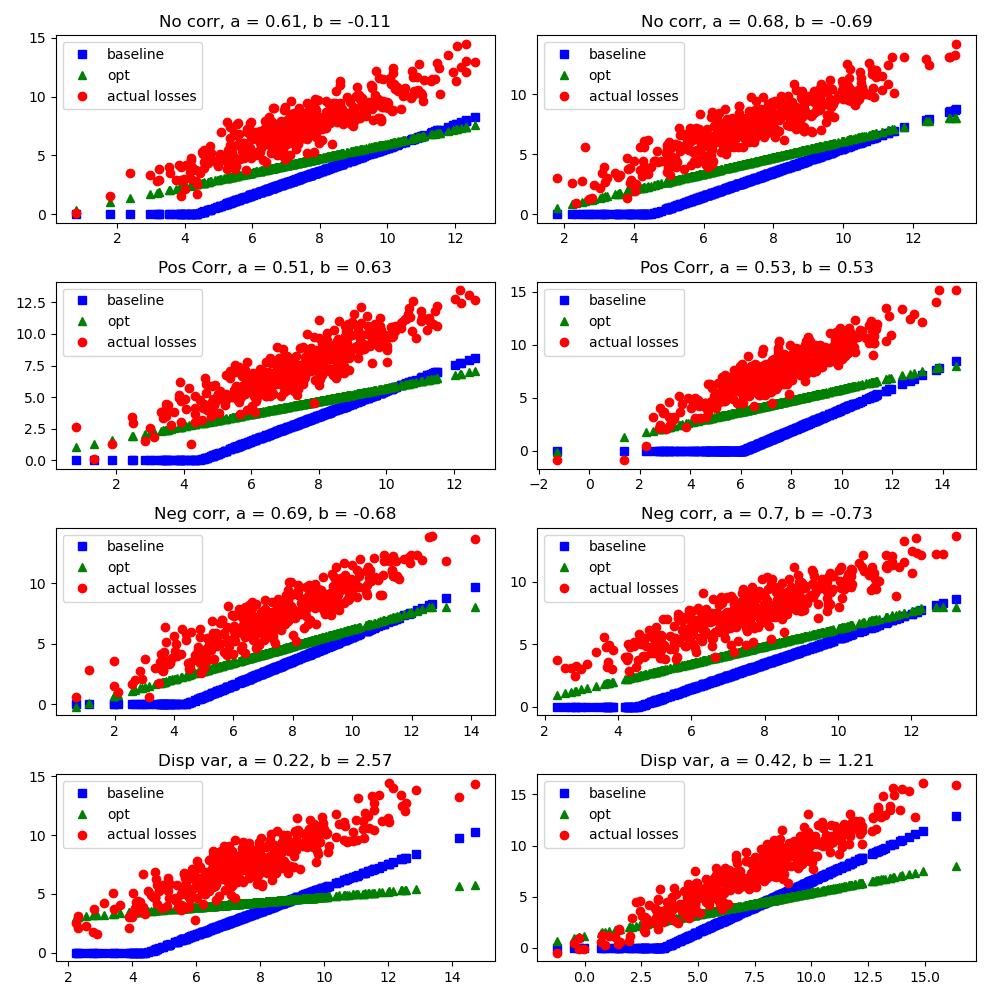
\includegraphics[width=0.75\textwidth]{../../output/figures/Exploration/scenario_exploration.png}
\end{figure}

\begin{figure}[H]
    \centering
    \caption{Scenario Payouts by Zone}
    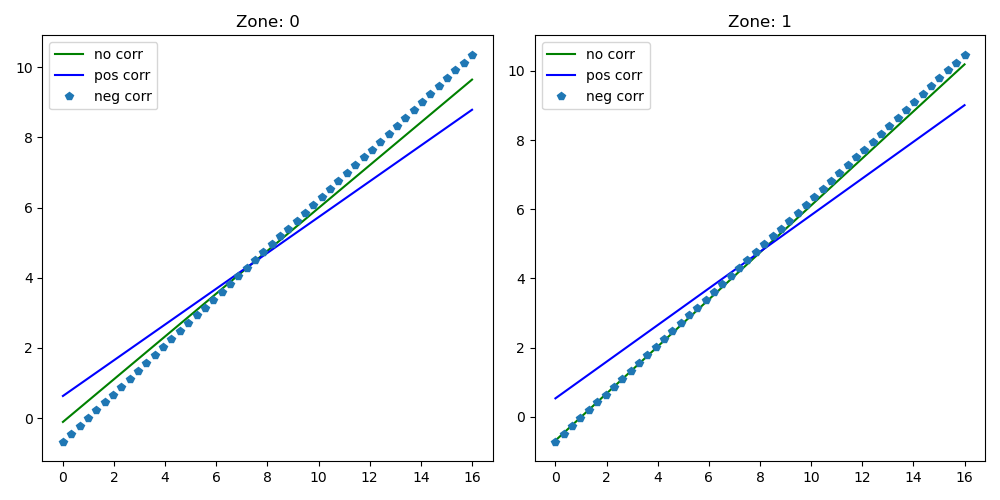
\includegraphics[width=0.75\textwidth]{../../output/figures/Exploration/scenario_payouts_by_zone.png}
\end{figure}


\section{Potential Next Steps}
\begin{itemize}
    \item Test how the different parameters affect the payout functions in the different scenarios
    \item Test a scenario where DGP is nonlinear
    \item Modify program to have an overall budget constraint, to make it easier to compare to the status quo. 
    \item Consider making deductible a decision variable
    \item Think about how to incorporate prediction uncertainty into the problem 
    \item Consider re introducing constraints. 
\end{itemize}

\end{document}